\documentclass[11pt]{article}

\usepackage{amsmath}
\usepackage{amssymb}
\usepackage{array}
\usepackage{geometry}
\usepackage{enumitem}
\usepackage{float}
\usepackage{cancel}
\usepackage{graphicx}
\usepackage[labelformat=empty]{caption}
\usepackage[T1]{fontenc}

\geometry{
	a4paper,
 	left=20mm,
 	top=20mm,
}

\setlength{\parindent}{0pt}

\begin{document}

\section{Matrizen}

\begin{description}[labelindent=16pt,style=multiline,leftmargin=4.5cm, noitemsep]
	\item[symmetrisch] $A^T = A$, quadratisch
	\item[schiefsymmetrisch] $A^T = -A$
	\item[hermitesch] $A^H = A$, quadratisch
	\item[unitär] $A^HA = I_n$ also $A^{-1} = A^H$
	\item[orthogonal] $A^TA = I_n$ also $A^{-1} = A^T$
\end{description}

\subsection{Regulär}

Sei $A^{m\times n}$ mit $m$ Gleichungen und $n$ Unbekannten \textbf{regulär} mit Rang $r$:
\begin{itemize}[noitemsep]
	\item $A$ ist quadratisch
	\item $r = n$
	\item $A$ ist invertierbar
	\item Die Zeilen- und Kolonnenvektoren sind linear unabhängig und erzeugen $\mathbb{E}^m$ bzw. $\mathbb{E}^n$
	\item $0$ ist kein Eigenwert
	\item $\det(A) \neq 0$
	\item Die lineare Abbildung $A$ ist bijektiv
	\item für jedes $b$ in $Ax = b$ gibt es genau eine Lösung
	\item die Kolonnen bilden eine Basis
\end{itemize}

\subsection{Multiplikation}

$A \cdot B = C$ ist definiert, falls $A$ gleichviele Kolonnen hat wie $B$ Zeilen. $C$ hat dann gleichviele Zeilen wie $A$ und gleichviele Kolonnen wie $B$.
	
\section{LR-Zerlegung}

\begin{equation*}
	Ax = b,\ PA = LR \Rightarrow Lc = Pb,\ Rx = c
\end{equation*}

\subsection{Pivotierung}
\begin{description}[noitemsep]
	\item
\end{description}

\section{Vektorräume}

\subsection{Vektor}

\begin{description}[labelindent=16pt,style=multiline,leftmargin=4.5cm, noitemsep]
	\item[Länge, 2-Norm] $||x|| :\equiv \sqrt{\langle x,x\rangle}$
	\item[Winkel] $\varphi = \arccos(\frac{\langle x,y\rangle}{||x|| ||y||}$
\end{description}

\subsection{Vektorräume}

\begin{description}[labelindent=16pt,style=multiline,leftmargin=5cm, noitemsep]
	\item[Unterraum] von $\text{span}\ S$ mit $S = {a_1,...,a_2}$ aufgespannt bzw. die Menge aller Linearkombinationen von $S$
	\item[Erzeugendensystem] die Menge $S$
	\item[Basis] linear unabhängiges Erzeugendensystem
	\item[Dimension] die Anzahl Basisvektoren
\end{description}

\section{Lineare Abbilungen}

Sei $F: X \mapsto Y$ mit $\dim X = n$ und $\dim Y = m$

\begin{description}[labelindent=16pt,style=multiline,leftmargin=5cm, noitemsep]
	\item[Matrixdarstellung] $A$, so dass $F(x) = Ax$
	\item[Kern] $\{x \in X; Fx = 0\}$, alle Vektoren in $X$, die auf $0$ zeigen
	\item[Bild] alle Vektoren in $Y$, die von $X$ mit $F$ erreicht werden
	\item[Rang] $\text{Rang}\ F :\equiv \dim \text{im}\ F$ \\ Dimension des Kolonnenraums \\ Dimension des Zeilenraums
	\item[Kolonnenraum] $\text{im}\ A = \mathcal{R}(A)$, der von den Kolonnen von $F$ aufgespannte Unterraum
	\item[Nullraum] $\text{ker}\ A = \mathcal{N}(A)$
\end{description}

Aus der \textbf{Dimensionsformel} $\dim X - \dim\ \text{ker}\ F = \text{Rang}\ F$ folgt, falls $F$:

\begin{description}[labelindent=16pt,style=multiline,leftmargin=7cm, noitemsep]
	\item[injektiv] keine Kollisionen \\ Kolonnenvektoren linear unabhängig \\ $\text{Rang}\ F = \dim X$ \\ $\text{ker}\ F = \{0\}$
	\item[surjektiv] es wird jedes Element in $Y$ erreicht \\ $\text{Rang}\ F = \dim Y$
	\item[bijektiv, d.h. Isomorphismus] $\text{Rang}\ F = \dim X = \dim Y$
	\item[bijektiv, d.h. Automorphismus] $\text{Rang}\ F = \dim\ X$ \\ $\text{ker}\ F = 0$
\end{description}

\subsection{Bestimmung der Basis für Kern/Bild}

\begin{enumerate}[noitemsep]
	\item Gauss anwenden
	\item Basis des \textbf{Bildes}
	\begin{enumerate}
		\item Alle linear unabhängigen Kolonnenvektoren (alle mit Pivot)
	\end{enumerate}
	\item Basis des \textbf{Kerns}
	\begin{enumerate}
		\item Setze $Fx = 0$
		\item Berechne von freien Variablen abhängige Lösung
		\item Klammere freie Variablen aus
	\end{enumerate}
\end{enumerate}

BEISPIEL TODO

\subsection{Bestimmung der Matrixdarstellung $A$ von $F$ bezüglich $B_X$ und $B_Y$}

\emph{Tipp:} Die Kolonnen von $A$ die Koordinatenvektoren der Bilder der Basisvektoren.
BEISPIEL TODO


\subsection{Transformation}
\begin{center}
	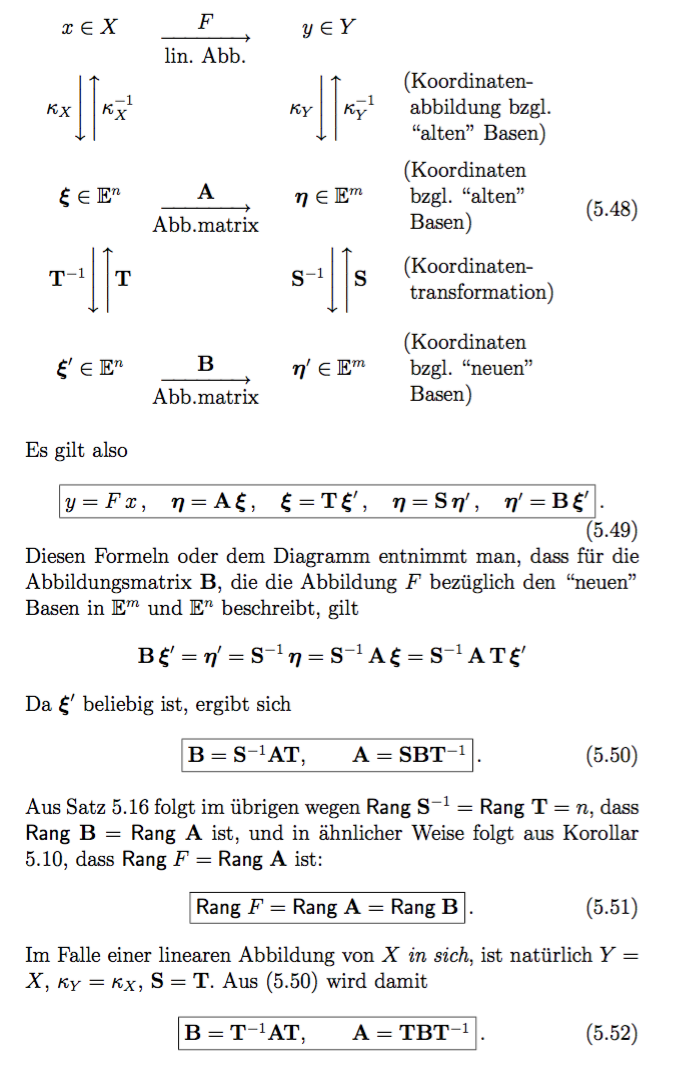
\includegraphics[width=400pt]{images/transformation}
\end{center}

\end{document}
